\section{Polynomial Hierarchy, Alternating TMs}

\subsection{Polynomial Hierarchy}

From \Cref{thm:relativizePandNP}, we have a notion of using {\P} and {\NP} with the power of oracle machines. However, we don't have a generalization of a ``hierarchy" of such oracle machines (the theorem only concerns the ``first level"). Therefore, in \cite{originalpolyhierarchypaper}, the notion of a ``polynomial hierarchy" was created. The hierarchy is defined (equivalently) as follows:
\begin{itemize}
\item $\Delta_0^\P = \Sigma_0^\text{\P}$ = $\Pi_0^\text{\P} = \text{\P}$,
\item $\Delta_i^\text{\P} = \text{\P}^{\Sigma_{i-1}^\text{\P}}$, 
\item $\Sigma_i^\text{\P} = \text{\NP}^{\Sigma_{i-1}^\text{\P}}$, 
\item $\Pi_i^\text{\P} = \text{\coNP}^{\Sigma_{i-1}^\text{\P}}$.
\end{itemize}

\begin{figure}
\label{fig:polyhierarchy}
\centering
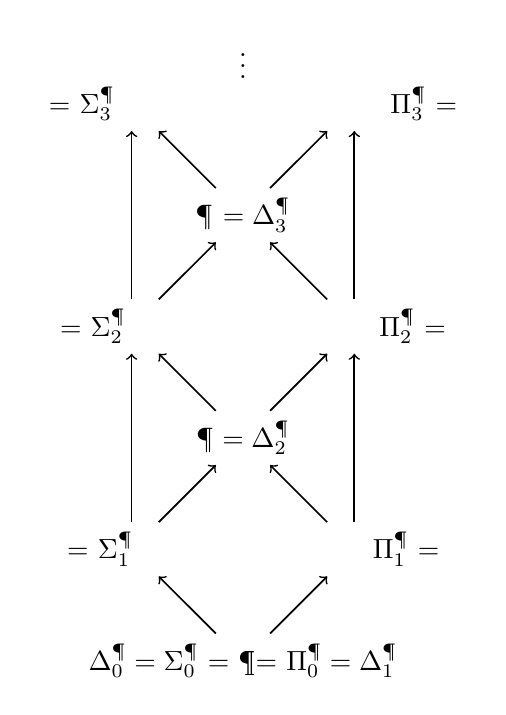
\begin{tikzpicture}[->, node distance=2cm, semithick]
 \node (P) {$\Delta_0^\P = \Sigma_0^\P$ = \P = $\Pi_0^\text{\P} = \Delta_1^\text{\P}$};
 \node (Sigma1) [above left of=P]       {{\NP} = $\Sigma_1^\text{\P}$ \hspace*{0.8cm}};
 \node (Pi1)    [above right of=P]      {\hspace*{1.2cm} $\Pi_1^\text{\P}$ = \coNP};
 \node (Delta2) [above left of=Pi1]     {$\text{\P}^\text{\NP} = \Delta_2^\text{\P}$ };
 \node (Sigma2) [above left of=Delta2]  {$\text{\NP}^\text{\NP}$ = $\Sigma_2^\text{\P}$ \hspace*{1.0cm}};
 \node (Pi2)    [above right of=Delta2] {\hspace*{1.5cm} $\Pi_2^\text{\P}$ = $\text{\coNP}^\text{\NP}$};
 \node (Delta3) [above left of=Pi2]     {$\text{\P}^{\text{\NP}^\text{\NP}} = \Delta_3^\text{\P}$};
 \node (Sigma3) [above left of=Delta3]  {$\text{\NP}^{\text{\NP}^\text{\NP}}$ = $\Sigma_3^\text{\P}$ \hspace*{1.3cm}};
 \node (Pi3)    [above right of=Delta3] {\hspace*{1.8cm} $\Pi_3^\text{\P}$ = $\text{\coNP}^{\text{\NP}^\text{\NP}}$};
 \node (dots)   [above of=Delta3]       {\vdots};
 \draw (P)      -> (Sigma1);
 \draw (P)      -> (Pi1);
 \draw (Sigma1) -> (Sigma2);
 \draw (Sigma1) -> (Delta2);
 \draw (Pi1)    -> (Pi2);
 \draw (Pi1)    -> (Delta2);
 \draw (Delta2) -> (Sigma2);
 \draw (Delta2) -> (Pi2);
 \draw (Sigma2) -> (Sigma3);
 \draw (Sigma2) -> (Delta3);
 \draw (Pi2)    -> (Pi3);
 \draw (Pi2)    -> (Delta3);
 \draw (Delta3) -> (Sigma3);
 \draw (Delta3) -> (Pi3);
\end{tikzpicture}
\caption{Polynomial Hierarchy, taken from http://commons.wikimedia.org/wiki/File:Polynomial\_time\_hierarchy.svg. Each arrow represents inclusion: for example, $\Sigma_1^\text{\P} \subseteq \Delta_2^\text{\P} \subseteq \Sigma_2^\text{\P}$.}
\end{figure}

\begin{definition}
The \emph{polynomial hierarchy}, called \PH, is defined to be:
\[
\PH = \bigcup_{k = 1}^{\infty} \Sigma_k^{\text{\P}}.
\]
\end{definition}

\begin{theorem}
$\PH$ can also be defined as:
\[
\PH = \bigcup_{k = 1}^{\infty} \Pi_k^{\text{\P}}.
\]
\end{theorem}

\begin{proof}
We have the simple inclusions: $\Sigma_i^\P \subseteq \Pi_{i+1}^\P \subseteq \Sigma_{i+2}^\P$.
\end{proof}

For $\PH$, we often call the $i$-th level of $\PH$ to be both $\Sigma_i^\text{\P}$ and $\Pi_i^\text{\P}$. A natural inclination, as has been done before with \NP, \PSPACE, \NL, and the like, is to find a complete problem for $\PH$. However, the following theorem shows that this is most likely not the case.

\begin{theorem}
If there is a $\PH$-complete language, then $\PH$ only has a finite number of levels.
\end{theorem}

\begin{proof}
Assume there exists a $\PH$-complete language, and let it be $L$. By definition, $\PH = \bigcup_{k = 1}^{\infty} \Sigma_k^{\text{\P}}$. Therefore, for some $j$, we have that $L \in \Sigma_j^\P$, and every language in \PH is polynomial-time reducible to $L$. However, any language $A$ that is polynomial-time reducible to some language $B \in \Sigma_j^\P$ has that $A \in \Sigma_j^\P$. Therefore, $\PH \subseteq \Sigma_j^\P$.
\end{proof}

\subsection{Alternating TMs}
\begin{definition}
\emph{Alternating TM}s (ATMs) are generalizations of NTMs, in that they behave the same as NTMs, but have an extra ``feature," that for every non-halting state, the state has a label from $\{\exists, \forall\}$. When running on some input, if the state has the $\exists$ label, then the ATM accepts if \emph{some} transition path from that state accepts; if the state has the $\forall$ label, then the ATM accepts if \emph{all} transition paths from that state accept.
\end{definition}